\documentclass{beamer}

%style
\mode<presentation>{
	\usetheme{Goettingen}
}
%packages
\usepackage[utf8]{inputenc}
\usepackage[ngerman]{babel}
\usepackage{graphicx}

%Einstellungen Präsentation
\title{Planeten}
\author{Nicolas Tobler}
\institute{Mathematisches Seminar 2018}
\date{014.05.2018}

%Bilder
\graphicspath{{Pictures/}}

%Beginn der Präsentation
\begin{document}

%Titelseite
\begin{frame}
\titlepage
\end{frame}

%Inhaltsverzeichnis
\begin{frame}
\frametitle{Inhalt}
\tableofcontents
\end{frame}

\section{Einführung}

\subsection{Planeten im Vergleich}
\begin{frame}
	\frametitle{Planeten im Vergleich}
	
	\begin{figure}
	\center
	\includegraphics[width=0.7\linewidth]{Pictures/planets.jpg}
	\end{figure}
	
\begin{columns}
\begin{column}{0.33\textwidth}
   Mars
   \begin{itemize}
   		\item[] Kaum Wolken
   		\item[] Heiss
   \end{itemize}
\end{column}
\begin{column}{0.33\textwidth}
   Venus
   \begin{itemize}
   		\item[] Dicke Wolkendecke
   		\item[] Heiss
   \end{itemize}
\end{column}
\begin{column}{0.33\textwidth}
   Erde
   \begin{itemize}
   		\item[] Normales Wetter
   \end{itemize}
\end{column}
\end{columns}
\end{frame}

\subsection{Motivation}
\begin{frame}
	\frametitle{Motivation}
	\begin{itemize}
		\item[] Normale Situation
	
		\pause
		\item[] El Niño
	
	\end{itemize}
\end{frame}


\section{Modell} 
\begin{frame}
	\frametitle{Modell}
	\begin{figure}
		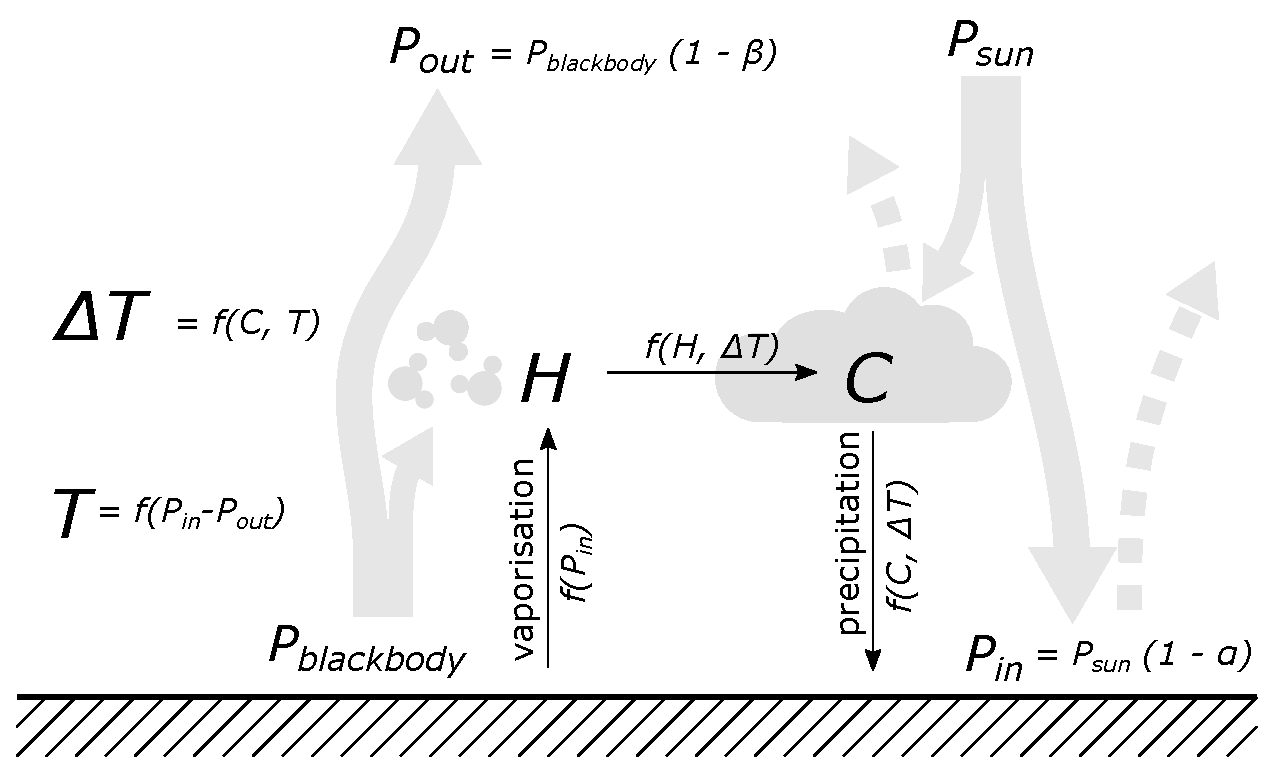
\includegraphics[width=\linewidth]{Pictures/Model.eps}
	\end{figure}
\end{frame}

\subsection{Energiehaushalt}
\begin{frame}
\frametitle{Energiehaushalt}
\begin{itemize}
	\item[] Absorbierte Leistung
	\begin{equation}
	P_{in} = \sigma T_{\astrosun}^4 \left( \frac{R_{\astrosun}}{a_{planet}} \right) ^2 \cdot (1-\alpha)
	\end{equation} 
	\item[] Abgestrahlte Leistung
	\begin{equation}
	P_{out} = (4 \pi R_{S}^2 \sigma T_{S}^4)(1 - \beta)
	\end{equation}
	\pause
	\item[] Albedo
	\begin{equation}
	\alpha(C) = (0.65 \cdot C) + 0.15;
	\end{equation}
	\pause
	\item[] Treibhauseffekt
	\begin{equation}
	\beta(H) = 0.5 \cdot H
	\end{equation}
\end{itemize}
\end{frame}

\subsection{Wasserkreislauf}
\begin{frame}
	\frametitle{Schrittweises Lösen einer DDE}
	\begin{itemize}
		\item[] Wolken
			\begin{equation}
			\dot{C} = p_4 \left( (H + H^5)(T_S - T_T) \right) - p_5 (C + C^5)
			\end{equation} 
			\pause
		\item[] Atmosphärischer Wasserdampf
			\begin{equation}
			\dot{H} = p_5 \left(P_{in} \right) - p_6 \left( (H + H^9 )(T_S - T_T) \right)
			\end{equation}
			\pause
		\item[] Lösung im Bereich von 0 bis 1 
		 	\pause
		 	\begin{equation}
		 	\dot{y}=-1 \textrm{   daraus folgt  } y=1-t
		 	\end{equation} 	
	\end{itemize}
\end{frame}

\subsection{Zusammengefasste Gleichungen}
\begin{frame}
\frametitle{Charakteristische Gleichung}
\begin{itemize}
	\item[] Beispiel
	\begin{equation}
	\dot{y}(t)=ky(t-\tau)
	\end{equation} 
	\item[] Ansatz
	\begin{equation}
	y(t) = ce^{\lambda t}
	\end{equation}
	\pause
	\item[] Einsetzen
	\begin{equation}
	\lambda ce^{\lambda t} = kce^{\lambda (t-\tau )}
	\end{equation} 	
	\pause
	\item[] Vereinfachen
	\begin{equation}
	\lambda  - ke^{-\lambda}= 0
	\end{equation}
\end{itemize}
\end{frame}

\section{Simulation}

\subsection{Chaotisches Verhalten}
\begin{frame}
	\frametitle{Chaotisches Verhalten ohne Dämpfungsterm}
	\begin{itemize}
		\item[] Gleichung ohne Dämpfung
			\begin{equation}
				\dot{T}(t)=-cT(t)+aT(t-\frac{1}{2}\tau_K)-bT(t-(\frac{1}{2}\tau_R+\tau_K))
			\end{equation}
			\pause
		\item[] Änderung des Parameters a
			\begin{figure}
				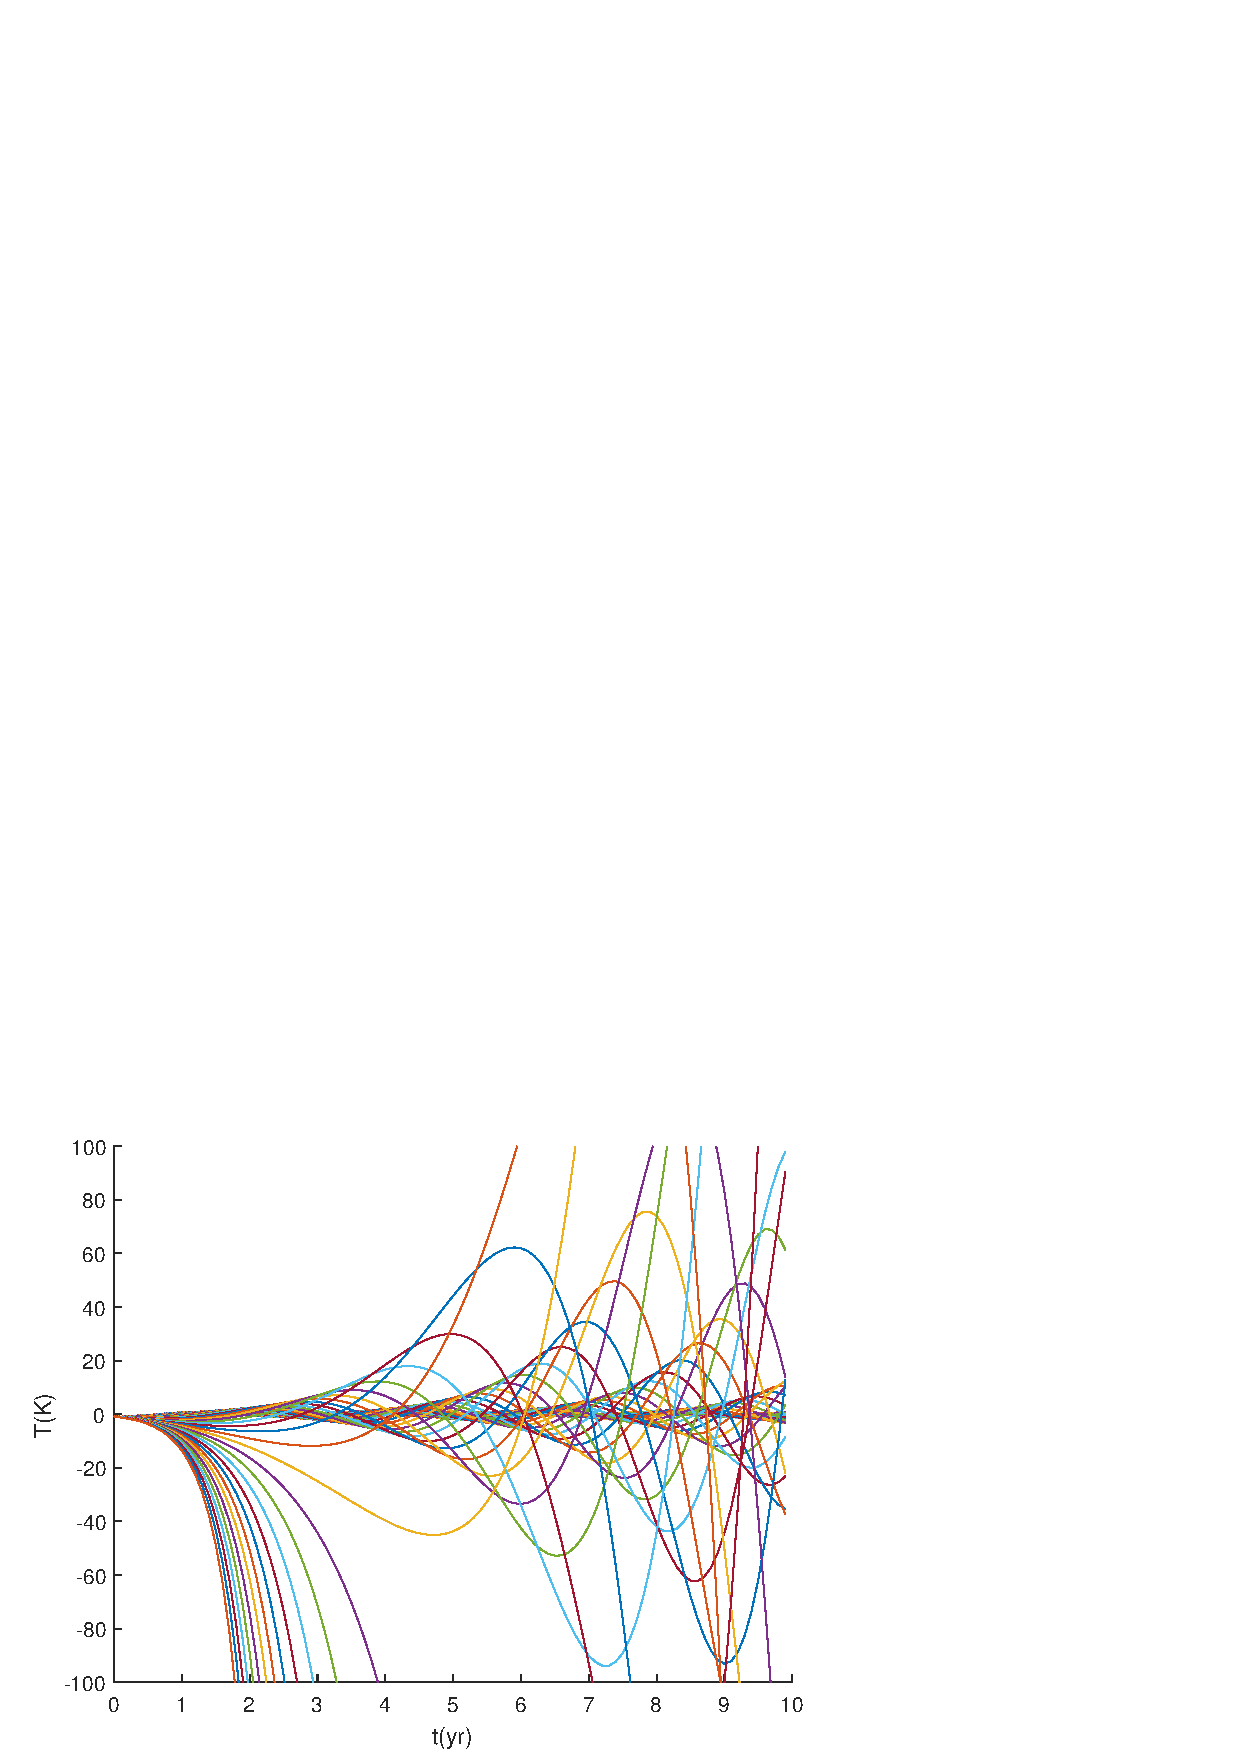
\includegraphics[width=0.9\linewidth, height=0.6\textheight]{param_a_e0.png}
			\end{figure}
	\end{itemize}
\end{frame}

\subsection{Vollständige Lösung}
\begin{frame}
\frametitle{Verhalten mit Dämpfungsterm}
\begin{itemize}
	\item[] Gleichung mit Dämpfung
	\begin{equation}
	\dot{T}(t)=-cT(t)+aT(t-\frac{1}{2}\tau_K)-bT(t-(\frac{1}{2}\tau_R+\tau_K))-\epsilon(T(t))^3
	\end{equation}
	\pause
	\item[] Änderung des Parameters a
	\begin{figure}
		\includegraphics[width=0.9\linewidth, height=0.6\textheight]{param_a.png}
	\end{figure}
\end{itemize}
\end{frame}

\subsection{Simulation}
\begin{frame}
\frametitle{Simulation und Vergleich mit realen Daten}
\begin{itemize}
	\item[] 
	\begin{figure}
		\includegraphics[width=0.9\linewidth, height=0.6\textheight]{Simulation_95_98.png}
	\end{figure}
	\item[] Anfangswertvektor und Vergleichsdaten von \url{http://www.cpc.ncep.noaa.gov/data/indices/sstoi.indices}
\end{itemize}
\end{frame}

\end{document}